% \begin{document}
\chapter{Variabili Aleatorie}
\section{Introduzione}
  Finora, abbiamo trattato solo di eventi, per i quali ci chiediamo, fatto l'esperimento aleatorio, se sono avvenuti o meno. Possiamo pensare di domandarci non se un'affermazione si realizza o meno, ma generalizzare l'idea e chiederci quale sara' la quantita' numerica aleatoria, associata quindi ad un esperimento. Vogliamo quindi formalizzare l'idea di una quantita' che dipende dall'esito di un esperimento aleatorio:
  \dfn{Variabile Aleatoria}{
    Diamo due affermazioni (come per gli eventi):
    \begin{itemize}
    \item \textbf{Affermazione}:

      Una variabile aleatoria e' un'affermazione che riguarda il risultato dell'esperimento aleatorio. Tale affermazione identifica uno e un solo numero, una volta noto l'esito. Stiamo quindi rispondendo alla domanda "Quanto vale ... ?"

      \item \textbf{Funzione}:

        Dato uno spazio di probabilita' $ (\Omega, \mathbb{P}) $ ed un insieme $ E \neq \emptyset $, si dice \textit{variabile aleatoria} ogni funzione $ X $ del tipo:
        \[
        X: \Omega \to E
        \]
        Se $ E = \mathbb{R} $, allora $ X $ e' una variabile aleatoria \textit{reale}. Puo' anche essere che $ E = \mathbb{R}^{n} $ con $ n > 1 $, e in questo caso si parla di variabili aleatorie \textit{vettoriali}.
      
    \end{itemize}
  }

  \ex{Lancio di due dadi}{
    Dato lo spazio di probabilita', definiamo una variabile aleatoria $ X $:
    \[
    X = \text{La somma dei due lanci}
    \]
    Dobbiamo, quindi, prendere l'esito dell'esperimento e sommare il valore dei due dadi. Questa operazione puo' essere vista come una funzione a cui viene passata l'esito dell'esperimento e che restituisce un numero reale:
    \begin{align*}
      X: \Omega \to \mathbb{R}
    \end{align*}
    Questa e' la definizione di variabile aleatoria come funzione.

    In questo caso, $ \Omega = \{1,...,6\}\times \{1,...,6\} = DR_{6,2} $, qundi:
    \[
      X((\omega_1, \omega_2)): \omega_1+\omega_2
    \]
  }
  \nt{
    Qualunque funzione da $ \Omega $ a $ \mathbb{R} $ e' una variabile aleatoria. Se $ \Omega $ e' piu' che numerabile sorgono dei problemi a causa dell'unione numerabile, quindi viene usata la $ \sigma $-algebra, un insieme delle parti ristretto per evitare tali problemi. 
  }

  \section{Variabili Aleatorie Costanti}
  Vediamo dei casi "banali" di variabili aleatorie per capire il loro funzionamento e come vengono definite. Iniziamo con le funzioni costanti:
  \dfn{Variabile Aleatoria Costante}{
    Una VA (variabile aleatoria) $ X $ si dice \textit{costante} se:
    \[
      \forall \omega \in \Omega.\ X(\omega) = a
    \]
    Dove $ a \in E $ e' un elemento fissato. E' definita $ \forall \Omega $, dato che e' deterministica (non dipende dall'esito dell'esperimento).
  }
  Come per gli eventi, anche le variabili aleatorie possono essere \textit{quasi} costanti:
  \dfn{Variabili Aleatorie Quasi Costanti}{
    Una VA $ X $ si dice \textit{quasi costante} se:
    \[
      \forall \omega \in \Omega.\ \mathbb{P}(X = a) = 1
    \]
  }
  \nt{
    La scrittura $ (X = a) $ e' una notazione che rappresenta l'evento $ A = \text{"Il valore di X sara' "} a $, ovvero il sottoinsieme di $ \Omega $ per cui tutti gli elementi, passati a $ X $, danno lo stesso valore $ a $, quindi:
    \[
      \mathbb{P}(X = a) \coloneq \mathbb{P}(\{\omega \in \Omega | X(\omega) = a\})
    \]
  }
  \ex{Lancio di un dado}{
    $ \Omega = \mathbb{R} $, $ \mathbb{P} $ probabilita' uniforme su $ \{1,...,6\} $ e nulla sul resto degli elementi.

    Con $ E = \mathbb{R} $, fisso $ a \in E $ e voglio costruire $ X: \Omega \to E $ tale che $ X $ e' quasi costante:
    \[
      X(\omega) = \begin{cases}
      a & \omega \in \{1,...,6\}\\
      \omega & \text{altrimenti}
      \end{cases}
    \]
    Questa e' effettivamente una VA quasi costante, dato che $ \mathbb{P}(X = a) = 1 $. Infatti abbiamo assegnato un valore costante $ a $ a tutti gli $ \omega $ la cui probabilita' non era nulla. Ricordiamoci che la notazione $ \mathbb{P}(X = a) $ puo' essere riscritta meglio come $ \mathbb{P}(\{\omega \in \Omega | X(\omega) = a\}) $, che in questo caso corrisponde con $ \mathbb{P}(\{1,...,6\}) $ che ovviamente e' uguale a 1.

    Notare che per tutti gli $ \omega $ con probabilita' nulla, il valore di $ X $ associato puo' essere qualunque cosa (non costante) e la $ X $ rimane comunque quasi costante. 
  }

  \section{Variabili Aleatorie Indicatrici (o di Bernulli)}

  \dfn{Varaibile Aleatoria Indicatirce}{
    Dato un evento $ A \subseteq \Omega $, definisco la variabile aleatoria indicatrice di $ A $ come:
    \[
      X(\omega): \mathbb{1}_A(\omega) = \begin{cases}
      1 & \omega \in A\\
      0 & \omega \notin A
      \end{cases}
    \]
  }
  Quindi, dato un evento, la VA indicatrice $ X $ ci \textit{indica} se l'esito $ \omega $ appartenga o meno all'evento. Notiamo che tutta l'informazione dell'evento $ A $ e' contenuta nella VA:
  \[
  A \rightsquigarrow \mathbb{1}_A
  \]
  Allora le VA sono \textit{generalizzazioni} del concetto di evento.

\ex{Prove ripetute e indipendenti}{
  Consideriamo uno schema di $n$ prove ripetute e indipendenti con probabilità di successo $p$, ossia uno spazio di probabilità discreto $(\Omega, P)$ in cui sono definiti $n$ eventi $C_1, \ldots, C_n$ indipendenti e con la stessa probabilità $p = P(C_i)$ (si ricordi il Paragrafo 1.3.4). Nel Paragrafo 1.3.4.3 abbiamo studiato gli eventi

  \begin{align*}
    A_k &:= \text{``esattamente $k$ prove hanno successo''}, \\
    B_\ell &:= \text{``il primo successo si verifica nella $\ell$-esima prova''},
  \end{align*}
    
  per $0 \leq k \leq n$ e $1 \leq \ell \leq n$. Introduciamo ora due variabili aleatorie
    
  \begin{align*}
    S &:= \text{``numero di successi nelle $n$ prove''}, \\
    T &:= \text{``prova in cui si ha il primo successo''},
  \end{align*}
    
  definite su $\Omega$ a valori rispettivamente in $\{0, 1, \ldots, n\}$ e in $\mathbb{N} \cup \{+\infty\}$, mediante
    
  \begin{equation}
    S(\omega) := \sum_{i=1}^{n} 1_{C_i}(\omega), \quad T(\omega) := \min\{i \in \{1, \ldots, n\} : \omega \in C_i\},
  \end{equation}
    
  con la convenzione $\min \emptyset := +\infty$. Possiamo allora esprimere gli eventi $A_k$ e $B_\ell$ nel modo seguente:
    
  \begin{equation}
    A_k = \{\omega \in \Omega : S(\omega) = k\}, \quad B_\ell = \{\omega \in \Omega : T(\omega) = \ell\}.
  \end{equation}
    
  Questo mostra che gli eventi $A_k$ e $B_\ell$ possono essere definiti in modo naturale in termini delle variabili aleatorie $S$ e $T$, specificandone un sottoinsieme di valori.
    
}

  \section{Eventi associati alle variabili aleatorie}

  Ma se io ho $ X $ variabile aleatoria, sono capace di risalire all'evento (o eventi) associati? Le variabili aleatorie sono generalizzazioni del concetto di evento, quindi data una variabile aleatoria ci sono una moltitudine di eventi associati (o generati)

  \dfn{Evento generato da una VA}{
    Sia $ X: \Omega \to E $ una VA. $\forall A \subseteq \mathbb{R} $ indichiamo con $ \{X \in A\} $ la controimmagine di $ A $ tramite $ X $:
    \[
      \{X \in A\} \coloneq X^{-1}(A) = \{\omega \in \Omega | X(\omega) \in A\}
    \]
    Quindi $ \{X \in A\} \subseteq \Omega $ e' un evento, ed e' costituito da tutti e soli gli esiti $ \omega $ per cui $ X(\omega) \in A $.

    Gli eventi di questo tipo si dicono \textit{generati da} $ X $.
  }

  \nt{
    La scrittura $ \{X = a\} $ che abbiamo usato prima e' equivalente a scrivere $ \{X \in \{a\}\} $. Allo stesso modo, possiamo considerare un intervallo di valori usando le disequazioni: $ \{X > a\} \equiv \{X \in (a,+\infty)\} $.
  }

  Segue quindi:
  \dfn{Insieme di eventi generati da una VA}{
    Data una VA $ X $, l'insieme degli eventi da essa generati si indica con:
    \[
      \sigma(X) \coloneq \{\{X \in A\} | A \subseteq \mathbb{R}\} \subseteq \powerset(\Omega)
    \]
  }

  \nt{
    $ \forall X: \Omega \to \mathbb{R} $ v.a. possiamo scrivere:
    \[
    \Omega = \{X \in \mathbb{R}\}
    \]
    \[
    \emptyset = \{X \in \emptyset\}
    \]
  }

  Calcoliamo l'insieme degli eventi generati dalle VA particolari che abbiamo visto:

  \begin{itemize}
  \item $ X $ \textbf{costante}:

    Fisso $ a \in \mathbb{R} $, tale che $ \forall \omega \in \Omega.\ X(\omega) = a $.

    $ \sigma(X) = ? $

    Fissato $ B \subseteq \mathbb{R} $, notiamo che ci sono solo due casi:
    \[
    \{X \in B\} = \begin{cases}
    \Omega & a \in B\\
    \emptyset & a \notin B
    \end{cases}
    \]
      Infatti, se $ a $ appartiene a $ B $ allora $ \forall \omega \in \Omega.\ X(\omega) \in B $ e quindi $ \{X \in B\} = \Omega $. Mentre se $ a $ non appartiene a $ B $, si ha che $ \forall \omega \in \Omega.\ X(\omega) \notin B $ e quindi $ \{X \in B\} = \emptyset $.
  \item $ X $ \textbf{indicativa}:

    Fisso $ A \subseteq \Omega $ tale che $ \forall \omega \in \Omega.\ X(\omega) = \mathbb{1}_A(\omega) $.

    $ \sigma(X) = ? $

    Fissato $ B \subseteq \mathbb{R} $, vediamo i casi:
      \[
      \{X \in B\} = \begin{cases}
      \Omega & 0 \in B \land 1 \in B\\
      \emptyset & 0 \notin B \land 1 \notin B\\
      A & 0 \notin B \land 1 \in B\\
      A^{c} & 0 \in B \land 1 \notin B
      \end{cases}
      \]
  \end{itemize}   

  \mprop{}{
    Sia $ X: \Omega \to \mathbb{R} $ VA su $ (\Omega, \mathbb{P}) $, allora $ \forall x \in \mathbb{R} $:
    \begin{enumerate}
      \item $ \mathbb{P}(\{X \geq a\}) = \mathbb{P}(\{X = a\}) + \mathbb{P}(\{X > a\}) $
      \item $ \mathbb{P}(\{X \geq a\}) = 1 - \mathbb{P}(\{X < a\}) $
    \end{enumerate}
  }
  \pf{}{
    \begin{enumerate}
      \item $ \{X \geq a\} = \{ \omega \in \Omega | X(\omega) > a \lor X(\omega) = a\} = \{X > a\} \uplus \{X = a\} $ dato che se $ X(\omega) > a $ allora $ X(\omega) \neq a $ e viceversa. Quindi l'equazione e' dimostrata per addittivita' finita.
      \item Dimostriamo che $ \{X \geq a\} $ e $ \{X < a\} $ sono complementari. Se $ X(\omega) \not\geq a $, allora $ X(\omega) < a $ e viceversa, fatto.
    \end{enumerate}
  }

   Possiamo confronare intervalli su $ \mathbb{R} $ per calcolare probailita'

 \section{Distribuzione (o legge) di una Variabile Aleatoria}

 Ora che sappiamo trovare l'evento generato da una variabile aleatoria e un sottoinsieme del suo codominio, possiamo calcolare la probabilita' di tale evento: 

 \dfn{Distribuzione di una VA}{
   Dati $ (\Omega, \mathbb{P}) $ e $ X: \Omega\to \mathbb{R} $ VA, chiamiamo legge di $ X $ la funzione:
   \begin{align*}
     \mathbb{P}_X: \powerset(\mathbb{R}) &\to [0,1]\\
     B &\mapsto \mathbb{P}(X \in B)
   \end{align*}
   Si scrive $ X \sim \mathbb{P}_X $ e si legge "$ X $ ha legge $ \mathbb{P}_X $".
 }
 \mprop{}{
   La distribuzione $ \mathbb{P}_X $ di una variabile aleatoria $ X: \Omega \to E $ e' una probabilita' sull'insieme $ E $. (per noi $ E $ sara' quasi sempre $ \mathbb{R} $).
 }
 La legge di una VA ne calcola quindi, dato un insieme di valori reali, la probabilita' che $ X(\omega) $ appartenga a tale intervallo. Quindi, anche senza conoscere la funzione $ X $, se conosciamo la sua distribuzione sappiamo quali valori puo' assumere e con quale probabilita'.

 Andiamo a costruire le distribuzioni delle VA "banali" studiate precedentemente:
  \begin{itemize}
  \item Variabili Costanti:

    $ a \in \mathbb{R}, X(\omega) = a.\ \forall \omega \in \Omega $

    \[
    B \subseteq \mathbb{R}.\ \{X \in B\} = \begin{cases}
    \Omega & a \in B\\
    \emptyset &  a \notin B
    \end{cases}
    \]
    \[
    \mathbb{P}_X(B) = \mathbb{P}(X \in B) = \begin{cases}
    1 & a \in B\\
    0 & a \notin B
    \end{cases}
    \]
      Questa e' la delta di Dirac di $ a $ valutata su $ B $
    \item Variabili Indicatrici:

      $ A \subseteq \Omega $, $ X(\omega) = \mathbb{1}_A(\omega) $
      \[
      B \subseteq \mathbb{R}, \{X \in B\} = \begin{cases}
      \Omega & 1, 0 \in B\\
      \emptyset & 1, 0 \notin B\\
      A & 1 \in B \land 0 \notin B\\
      A^{c} & 1 \notin B \land 0 \in B
      \end{cases}
      \]
      \[
        P_X(B) = P(X \in B) = \begin{cases}
        1 & 1,0 \in B\\
        0 & 1,0 \notin B\\
          P(A) & 1 \in B \land 0 \notin B\\
          1-P(A) & 1 \notin B \land 0 \in B
        \end{cases}
      \]
      Questa e' una probabilita' discreta, quidni e' possibile crearla usando una combinazione lineare di delta di Dirac: 
      \[
        = P(A)\delta_1(B) + (1-P(A))\delta_0(B)
      \]
      Ovvero:
      \[
        P_X(\cdot) = P(A)\delta_1(\cdot) + (1-P(A))\delta_0(\cdot)
      \]
      Distribuzione (o legge) di Bernulli. Se la variabile aleatoria diventa piu' complicata, aumentano il numero di delta.
\dfn{Distribuzioni di Bernulle}{
  $\P_x (\cdot) = \P(A) \delta_1(\cdot) + (1-\P(A))\delta_0(\cdot)$
}
  \end{itemize}

  \section{Funzione di Ripartizione}
  Molto bella la distribuzione di una VA, ma prende come input insiemi (sottoinsiemi di $ \mathbb{R} $) e questo ci complica un po' la vita. Vediamo una caratterizzazione piu' semplice che ci aiutera soprattutto per le VA assolutamente continue:
  \dfn{Funzione di Ripartizione}{
    Dati $ (\Omega, P) $ SP e una VA $ X: \Omega \to \mathbb{R} $, si chiama \textit{funzione di ripartizione} o \textit{CDF} di $ X $ la funzione:
    \begin{align*}
      F_X: \mathbb{R} &\to [0,1]\\
      x &\mapsto P_X((-\infty, x]) = P(X \leq x)
    \end{align*}
  }
 Diamo un'occhiata a come sono definite le funzioni di ripartizione per i soliti due casi "banali" di VA:
 \begin{itemize}
 \item VA Costanti:

   $ X(\omega) = a \implies P_X(B) = \delta_a(B) $, quindi la relativa funzione di ripartizione sara': 
  \[
  F_X(n) = P_X((-\infty, n]) = \delta_a(\{-\infty, n]) = \begin{cases}
  1 & n \geq a\\
  0 & n < a
  \end{cases}
  \]
    \begin{center}
      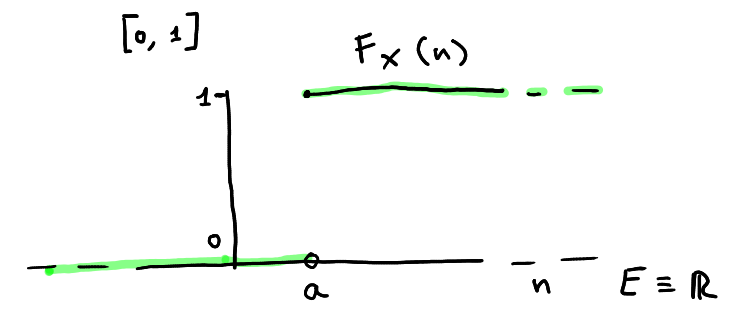
\includegraphics[width=0.5\textwidth]{img/2025-03-31-17-00-15.png}
    \end{center}
\item VA Indicatrici:

  $ X(\omega) = \mathbb{1}_A \implies P_X(B) = P(A)\delta_1(B) + (1-P(A))\delta_0(B) $, quindi la relativa funzione di ripartizione sara':
    \[
      F_X(x) = P_X((-\infty, x]) = P(A)\delta_1((-\infty, x]) + (1-P(A))\delta_0((-\infty, x])
    \]
     \[
     = \begin{cases}
     1 & x \geq 1\\
       1-P(A) & 0 \leq x < 1\\
     0 & x < 0
     \end{cases}
     \]
     \begin{center}
       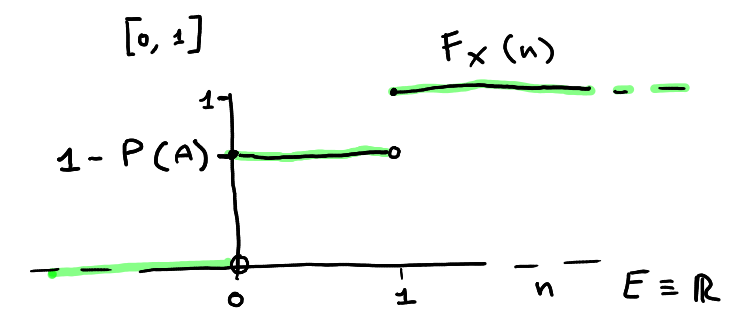
\includegraphics[width=0.5\textwidth]{img/2025-03-31-17-13-24.png}
     \end{center}
 \end{itemize}

Teorema datoci dalla Shlein, che ci caratterizza la funzione di ripartizione:
\thm{Teorema di Teodoro}{
  $ (\Omega, P) $ SP, $ X: \Omega \to \mathbb{R} $, $ F_X $ fdr, allora:
  \begin{enumerate}
  \item $ F_X $ e' monotona crescente
  \item $ F_X $ e' continua a destra, ovvero $ \forall n \in \mathbb{R}.\ \lim_{y\to x^{+}} F_X(y) = F_X(n) $
  \item  $ \lim_{n \to +\infty} F_X(n) = 1 $
  \item $ \lim_{n\to -\infty} F_X(n) = 0 $
  \end{enumerate}

  Vale anche il viceversa: se $ G: \mathbb{R} \to [0,1] $ verifica 1,2,3,4, allora
  \[
    \exists(\Omega, P), X:\Omega\to \mathbb{R}.\ G \equiv F_X
  \]
}
\pf{}{
  \begin{itemize}
    \item 1) Devo dimostrare che $ \forall x,y \in \mathbb{R}, x < y.\ F_X(x) \leq F_X(y) $, ovvero che $ P_X((-\infty, x]) \leq P_X((-\infty, y]) $. Dato che $ (-\infty, n] \subset (-\infty, y] $ e col fatto che $ P_X $ e' una probabilia', e' dimostrabile usando la proprieta' di monotonia delle probabilita'.
    \item 2) 3) 4) Per queste dimostrazioni serve dimostrare prima la \textit{Stabilita' della Probabilita' per limiti monotoni}:
  \end{itemize}
}
\mlenma{}{
  Sia $ (\Omega, P) $ SP
  \begin{itemize}
    \item Data $ "A_x \uparrow A" $, ovvero una successione di eventi tali che $ A_x \subset A_{x+1}, \bigcup_{x=1}^{+\infty} A_x = A $, allora:
      \[
        \lim_{x\to+\infty} P(A_x) = P(A)
      \]
    \item Data $ "A_x \downarrow A" $, ovvero una successione di eventi tali che $ A_x \supset A_{x+1}, \bigcap_{x=1}^{+\infty} A_x = A $, allora:
      \[
        \lim_{x\to+\infty} P(A_x) = P(A)
      \]
  \end{itemize}

  Stessa roba per monotona al contrario
}
  Dato questo lemma, che non dimostriamo perche' si, possiamo concludere la dimostrazione precedente:
  \pf{}{
    3) Dobbiamo dimostrare che $ \lim_{x\to+\infty} P_X((-\infty, x]) = 1 $. Usiamo il lemma appena introdotto, dato che se poniamo $ A_x = (-\infty, x) $, possiamo creare una successione tale che $ A_x \uparrow \mathbb{R} $, per cui $ \lim_{x\to+\infty} P_X(A_x) = P_X(\mathbb{R}) = 1 $.

    Gli altri punti sono lasciati al DarioDestroyer04 come compito per casa
  }

    $ F_X $ e' continua a destra, quindi $ \lim_{y \to x^{+}}F_X(y) = F_X(x) = P(X \leq x)$. Inoltre si puo' dimostrare (usando il lemma) che esiste anche il limite sinistro e vale:
    \[
      \lim_{y\to x^{-}} F_X(y) = P(X < x)\ (F_X(x^{-}))
    \]
    Inoltre, sappiamo che:
    \[
      \underbrace{P(X \leq x)}_{F_X(x)} = \underbrace{P(X < x)}_{F_X(x^{-})} + \underbrace{P(X = x)}_{\Delta F_X(x)}
    \]
    \begin{center}
      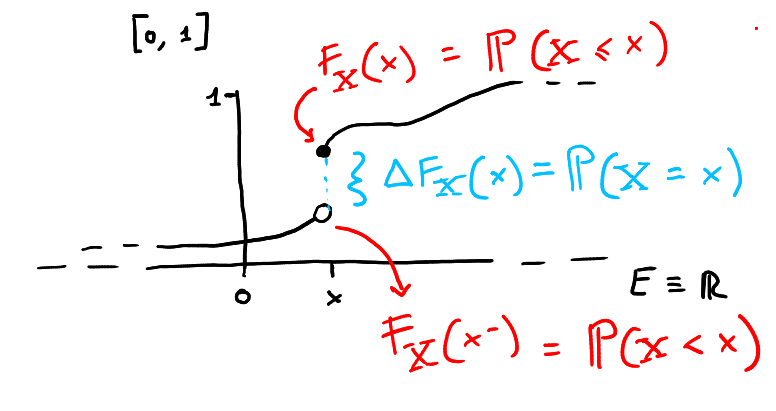
\includegraphics[width=0.5\textwidth]{img/2025-03-31-19-35-15.png}
    \end{center}

    Quindi possiamo calcolare la probabilita' di ogni intervallo in termini della $ F_X $:
    \begin{itemize}
      \item $ (a,b] $: $ P_X((a,b]) = F_X(b) - F_X(a) $
      \item $ [a,b) $: $ P_X([a,b)) = F_X(b^{-}) - F_X(a^{-}) $
      \item $ (a,b) $: $ P_X((a,b)) = F_X(b^{-}) - F_X(a) $
      \item $ [a,b] $: $ P_X([a,b]) = F_X(b) - F_X(a^{-}) $
    \end{itemize}

 \nt{
   Conoscere $ \mathbb{P}_X $ $ \forall B \subseteq \mathbb{R} \iff$  conoscere $ \mathbb{P}_X $ $ \forall I $ intervallo di $ \mathbb{R} $, dato che:
   \begin{itemize}
   \item Ogni intervallo e' anche un'insieme
    \item Dato un sottoinsieme di $ \mathbb{R} $, questo puo' sempre essere scritto come unione di intervalli
   \end{itemize}

   Quindi, $F_X$ \textbf{determina completamente la distribuzione} di $X$, dato che ci da la distribuzione per tutti gli intervalli, e quindi per tutti gli insiemi.
 }

 \section{Variabili Aleatorie Discrete}

 Dato che ci stiamo concentrando sulle probabilita' discrete, ci conviene applicare la definizione \ref{dfn:probDiscr} anche per le VA:
 \dfn{Variabile Aleatoria Discreta}{
   Una VA $ X: \Omega \to E $ definita su uno spazio di probabilita' $ (\Omega, P) $ e' detta \textit{discreta} se esiste un sottoinsieme $ S_X \subset Im(X) $ finito o numerabile tale che:
   \[
     P_X(S_X) \coloneq P(X \in S_X) = 1
   \]
   Quindi un VA e' discreta sse la sua distribuzione e' una probabilita' discreta.

   Il sottoinsieme $ S_X $ e' chiamato supporto di $ X $.
 }

 \nt{
   Se $ \Omega $ o $ E $ sono finiti o numerabili, allora una VA definita su di essi sara' sicuramente discreto.
 }

 \subsection{Caratterizzazione delle VA discrete}
 Che relazione esiste tra $ p_X $ e la distribuzione di $ X $ ($ P_X $)? E tra $ p_X $ e $ F_X $?
 \subsubsection{Distribuzione}
 Essendo $ P_X $ una probabilita' discreta, possiamo definirla usando la Delta di Dirac:

 Sia $ S_X = \{x_1,...,x_n\} $ il supporto di $ X $, allora $ \exists p_1,...,p_n \in (0,1], \sum_{i=1}^{n} p_i = 1 $ tale che:
 \[
   \forall B \subseteq E.\ P_X(B) = \sum_{i=1}^{n} p_i \delta_{x_i}(B)
 \]
 Per definizione di $ P_X $, sappiamo che $ \forall x \in E $:
 \[
   P_X(\{x\}) = P(X = x)
 \]
 Per cui, mettendo insieme le due definizioni:
 \[
   \forall x_i \in S_X.\ P_X(\{x_i\}) = \sum_{j=1}^{n} p_j \underbrace{\delta_{x_j}(\{x_i\})}_{\text{vale 1 solo quando } j = i} = p_i = P(X = x_i)
 \]
 Quindi $ \forall x_i \in S_X.\  p_i = P(X = x_i) $ e possiamo dire che $ X $ e' una VA discreta se e solo se:
 \[
   \forall B \subseteq E.\ P_X(B) = \sum_{i=1}^{n} P(X = x_i)
 \]
Dato che sara' una scrittura ricorrente, definiamo:
\dfn{Densita' discreta di una VA}{
  Data una VA discreta $ X $, si definisce \textit{densita' discreta} di $ X $ la funzione:
  \begin{align*}
    p_X: \mathbb{R} &\to [0,1]\\
    x &\mapsto P_X(\{x\}) = P(X = x)
  \end{align*}
}

Possiamo quindi scrivere
\[
  \forall B \subseteq E.\ P_X(B) = \sum_{i=1}^{n} p_X(x_i)
\]
 
\subsubsection{Funzione di Ripartizione}
Ricordiamo che possiamo esprimere $ F_X(x) $ come $ P_X((-\infty, x]) $ per tutti i valori di $ x $. Quindi, per quanto abbiamo detto sopra:
\[
  F_X(x) = \sum_{x_i \in (-\infty, x]} p_X(x_i)\delta_{x_i}((-\infty, x]) \quad \forall x \in \mathbb{R}
\]
Ma se $ x_i \notin S_X $, allora $ p_X(x_i) = 0 $, quindi:
\begin{itemize}
  \item Se $ \forall x_i \in S_X.\ x < x_i $, allora $ F_X(x) = 0 $
  \item Altrimenti, $ F_X(x) = \sum_{x_i \in S_X.\ x_i \leq x} p_X(x_i) $
\end{itemize}
Cio' significa che il valore della fdr cambia solo nei punti del supporto, dove abbiamo dei "salti" del valore $ p_X(x_i) $, mentre del resto e' costante.

\subsubsection{Conclusioni}
\thm{Caratterizzazione della distribuzione e fdr di una VA discreta tramite la sua densita'}{
  Sia $ X $ una VA su $ (\Omega, P) $, le seguenti affermazioni sono equivalenti:
  \begin{enumerate}
  \item $ X $ e' VA discreta con supporto $ S_X $ e densita' $ p_X $
  \item $ X $ ha fdr $ F_X $ \textbf{costante a tratti}: e' costante tranne nei punti di $ S_X = \{x_1,...,x_n\} $, in cui $ F_X $ "salta" con ampiezza
    \[
    \Delta F_X(x) = F_X(x) - F_X(x^-) = p_X(x) 
    \]
      La fdr ha quindi la seguente forma:
      \[
    F_X(x) =
    \begin{cases}
    0 & x < x_1, \\
    p_1 & x_1 \leq x < x_2, \\
    p_1 + p_2 & x_2 \leq x < x_3, \\
    \vdots & \vdots \\
    1 & x \geq x_n.
    \end{cases}
    \]

    % Esempio di grafico
    \begin{center} % TODO: sistemare
      
      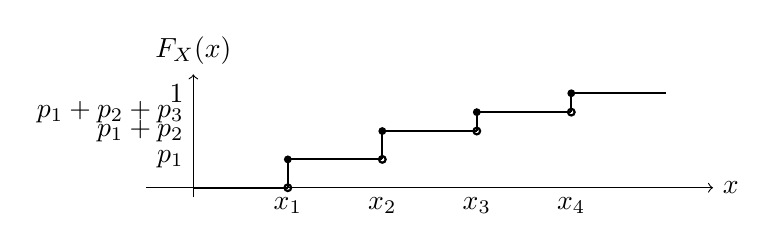
\begin{tikzpicture}[scale=1.2]
        % Assi
        \draw[->] (-0.5, 0) -- (5.5, 0) node[right] {$x$};
        \draw[->] (0, -0.1) -- (0, 1.2) node[above] {$F_X(x)$};
        
        % Punti di salto
        \draw[thick] (0, 0) -- (1, 0);
        \draw[thick] (1, 0) -- (1, 0.3);
        \draw[thick] (1, 0.3) -- (2, 0.3);
        \draw[thick] (2, 0.3) -- (2, 0.6);
        \draw[thick] (2, 0.6) -- (3, 0.6);
        \draw[thick] (3, 0.6) -- (3, 0.8);
        \draw[thick] (3, 0.8) -- (4, 0.8);
        \draw[thick] (4, 0.8) -- (4, 1);
        \draw[thick] (4, 1) -- (5, 1);
        
        % Punti
        \filldraw[black] (1, 0.3) circle (1pt);
        \filldraw[black] (2, 0.6) circle (1pt);
        \filldraw[black] (3, 0.8) circle (1pt);
        \filldraw[black] (4, 1) circle (1pt);
        
        % Cerchi vuoti
        \draw[thick] (1, 0) circle (1pt);
        \draw[thick] (2, 0.3) circle (1pt);
        \draw[thick] (3, 0.6) circle (1pt);
        \draw[thick] (4, 0.8) circle (1pt);

        % Etichette
        \node[below] at (1, 0) {$x_1$};
        \node[below] at (2, 0) {$x_2$};
        \node[below] at (3, 0) {$x_3$};
        \node[below] at (4, 0) {$x_4$};
        \node[left] at (0, 0.3) {$p_1$};
        \node[left] at (0, 0.6) {$p_1 
        + p_2$};
        \node[left] at (0, 0.8) {$p_1 + p_2 + p_3$};
        \node[left] at (0, 1) {$1$};
      \end{tikzpicture}
  \end{center}
      Quindi $ F_X $ e' data dalla formula:
      \[
        F_X(x) = \sum_{x_i \in S_X.\ x_i \leq x} p_X(x_i),\quad \forall x \in \mathbb{R}
      \]
    \item se $B$ è un sottoinsieme dei possibili valori di $X$ (anche con probabilita' nulla), allora:
  \begin{equation}
    \P(X\in B) = \P_X(B) = \sum_{x_i\in B}p_X(x) = \sum_{x_i\in B}\Delta F_X(x_i)
  \end{equation}
  \end{enumerate}
}

\ex{Esercizio Riassuntivo (2.1 libro)}{
  Sia $ G: \mathbb{R} \to [0,1] $ una funzione data da:
  \[
    G(x) = \begin{cases}
    0 & x < 0\\
    1/2 & 0\leq x < 1\\
    2/3 & 1\leq x<2\\
    11/12 & 2\leq x < 3\\
    1 & x\geq 3
    \end{cases}
  \]
  \begin{enumerate}
  \item Mostrare che $ G $ e' una funzione di ripartizione.
  \item Mostrare che $ X $ e' discreta. Determinare supporto e densita' discreta di $ X $.
  \item Trovare $ P_X $
  \item Calcolare $ P(X > 1/2), P(2 < X \leq 4), P(1< X<2), P(X < 3) $.
  \item Mostrare che $ Y = (X-2)^2 $ e' una variabile aleatoria discreta. Determinare $ S_Y e p_Y $.
  \end{enumerate}
  \textbf{Soluzione}:
  \begin{enumerate}
  \item Dobbiamo dimostrare che $ G $ ha le quattro proprieta' delle funzioni di ripartizione:
    \begin{itemize}
    \item E' ovviamente monotona crescente
    \item In tutti i punti di discontinuita', e' sempre continua a dx ($ \lim_{x\to k^{+}} G(x) = k $)
    \item I limiti a sx e dx sono 0 e 1
    \end{itemize}
    Quindi $ G $ e' una funzione di ripartizione.
    \item Essendo $ F_X(x) $ costante a tratti, $ X $ e' per forza discreta con supporto $ S_X = \{0, 1, 2, 3\} $.

      La densita' discreta $ p_X(x) $ si calcola guardando il "salto" di $ F_X(x) $ nel punto $ x $:
      \[
        \forall x \in S_X.\ p_X(x) = F_X(x) - F_X(x^{-}) = \Delta F_X(x)
      \]
      TODO: fare graficuccio e tabellonski
    \item Per la caratterizzazione della distribuzione usando la densita:
      \[
        P_X(B) = \sum_{x \in S_X} p_X(x)\delta_x(B)
      \]
    \item Va beh usa il punto prima per fare sta roba
    \item $ Y $ e' una VA che puo' essere riscritta come una composizione fra una funzione $ Z: \mathbb{R} \to \mathbb{R}.\ Z(x) = (x-2)^2 $ e $ X $. Per questo motivo, se $ X $ ha lo stesso valore per degli $ \omega \in \Omega $, allora anche in $ Y $ quegli $ \omega $ avranno la stessa immagine. Ovvero, $ |Im(Y)| \leq |Im(X)| $, che implica che $ |S_Y| \leq |S_X| $. In piu', possiamo dire che:
      \[
        p_Y(y) = \sum_{x \in Z^{-1}(y)} p_X(x) \quad \forall y \in \mathbb{R}
      \]
      Quindi $ S_Y = \{y \in \mathbb{R} | \exists x \in S_X.\ y = Z(x)\} $ TODO: molte di ste cose non le ho dimostrate/spiegate bene, forse sarebbe meglio farlo prima?
  \end{enumerate}
}
\section{Indici di sintesi di una distribuzione}

La distribuzione di una VA discreta puo' essere descritta in maniera sintetica tramite due quantita' numeriche: 
\begin{itemize}
\item La \textit{media}, che indica il valore "centrale" della distribuzione, ovvero il valore medio di $ X $ pesato con le probabilita' di ogni valore
\item La \textit{varianza}, che e' un indice di dispersione, ossia ci dice quanto quanto la distribuzione si concentra attorno alla media
\end{itemize}

\subsection{Media o valore atteso}
\dfn{Valore atteso di una variabile aleatoria}{
  Se $X$ è una variabile aleatoria discreta con densità di probabilità $p_X$, allora il valore atteso di $X$ è:
  \[
    E[X] \coloneq \sum_{x\in S_X} x p_X(x)
  \]
}
\nt{
  \begin{align*}
    \mathbb{E}[X - \mathbb{E}[X]] &= \mathbb{E}[X] - \mathbb{E}[\mathbb{E}[X]]\\
    &= \mathbb{E}[X] - \mathbb{E}[X] = 0
  \end{align*}
}
\thm{Stabilita' delle VA con composizione}{
  Sia $X$ una variabile aleatoria discreta con densità di probabilità $p_X$ e sia $g:\mathbb{R}\to \mathbb{R}$ una funzione. Allora il valore atteso di $g(X)$ è:
  \[
    \mathbb{E}[g(X)] = \sum_{x\in S_X} g(x)p_X(x)
  \]
}
\mprop{Linearita' del Valore atteso}{
  Siano $ X,Y $ VA discrete, allora $ \forall \alpha, \beta \in \mathbb{R} $:
  \[
    \mathbb{E}[\alpha \cdot X + \beta \cdot Y] = \alpha \mathbb{E}[X] + \beta \mathbb{E}[Y]
  \]
}
\pf{Dimostrazione}{
  Il bro fa una dimostrazione prendendo un solo caso, non ho capito TODO: boh
}

\subsection{Varianza}
\dfn{Varianza di $X$ }{
  Se $X$ è una variabile aleatoria discreta con densità di probabilità $p_X$ e valore atteso $E[X]$, allora la varianza di $X$ è:
  \[
    Var(X) = E[(X-E[X])^2] = \sum_{x\in S_X} (x-E[X])^2 p_X(x)
  \]
  La varianza e' anche indicata con $ \sigma^2 $.
}

\mprop{}{
  Si osservi che:
  \begin{align*}
    var(X) &= \mathbb{E}[X^2] - (\mathbb{E}[X])^2\\
    &= \sum_{x \in S_X} x^2 \cdot p_X(x) - \left( \sum_{x \in S_X} x \cdot p_X(x) \right)^2
  \end{align*}
}

\dfn{Deviazione standard}{
  Si definisce \textit{deviazione standard} la quantita':
  \[
    \sigma(X) \coloneq \sqrt{var(X)}
  \]
}
\nt{
  Se $ X $ e' una grandezza fisica espressa in una certa unita di misura, la deviazione standard ha il vantaggio di avere la stessa unita' di misura.
}
\section{Distribuzioni notevoli di VA discrete}

\subsection{Distribuzione uniforme discreta}
\dfn{Distribuzione uniforme discreta}{
  Una variabile aleatoria $X$ si dice avere una distribuzione uniforme discreta su un insieme di supporto $S_X = \{x_1, \dots, x_n\}$ di cardinalità $n$ se la densità di probabilità di $X$ è:
  \[
    p_X(x) = \frac{1}{n}, \quad \forall x\in S_X
  \]
  E si scrive $ X \sim Unif(\{x_1,...,x_n\}) $
}

Si può rappresentare questa distribuzione attraverso questa tabella:
\begin{center}
  \begin{tabular}{c|c|c|c|c|c}
    $X$ & $x_1$ & $x_2$ & $\dots$ & $x_n$ &  \\
    \hline
    $p_X(x)$ & $\frac{1}{n}$ & $\frac{1}{n}$ & $\dots$ & $\frac{1}{n}$ & 1\\ 
  \end{tabular}
\end{center}

In pratica il valore atteso di una variabile aleatoria con distribuzione uniforme discreta è:
\[
  E[X] = \sum_{x\in S_X} x p_X(x) = \sum_{x\in S_X} x \frac{1}{n} = \frac{1}{n}\sum_{x\in S_X} x = \frac{1}{n} \frac{n(n+1)}{2} = \frac{n+1}{2}
\]

mentre la varianza è:
\[
  Var(X) = \sum_{x\in S_X} (x-E[X])^2 p_X(x) = \frac{1}{n} \sum_{i=1}^n (x_i - E[X])^2
\]

\subsection{Distribuzione di Bernulli}
\dfn{Distribuzione di Bernulli di parametro $p\in [0,1]$}{
  Una variabile aleatoria $X$ con un insieme di supporto $S_X = \{ 0,1 \}$ si dice avere una distribuzione di Bernoulli di parametro $p$ se la sua densità di probabilità è:
  \[
    p_X(x) = 
    \begin{cases}
      p & \text{se } x=1,\\
      1-p & \text{se } x=0
    \end{cases}
  \]
}
Si può rappresentare questa distribuzione attraverso questa tabella:

\begin{center}
  \begin{tabular}{c|c|c|c}
    $X$ & 0 & 1& \\
    \hline
    $p_X(x)$ & $1-p$ & $p$ & 1\\ 
  \end{tabular}
\end{center}

Si noti che le variabili aleatorie di bernulli sono tutte Varaibili aleatorie indicatrici:
\[
  X = \mathbb{1}_A
\]
\[
  X(w) = \begin{cases}
    1 & w\in A\\
    0 & w\notin A
  \end{cases} \quad X \sim B(p)
\]

In pratica il valore atteso di una variabile aleatoria con distribuzione uniforme discreta è:
\[
  E[X] = \sum_{x \in S_X} x p_X(x) = 0 \cdot (1-p) + 1 \cdot p = p
\]
Mentre la sua varianza è:
\[
  Var(X) = E[X^2] - (E[X])^2 = p - p^2 = p(1-p)
\]

Si noti Inoltre che:
\[
  E[X^2] = \sum_i x_i^2 p_X (x_i) = 0 \cdot (1-p) + 1 \cdot p = p
\]

\subsection{Distribuzione binomiale di parametri $ p \in [0,1] $ e $ n \in \mathbb{N} $}
Si consideri ora una generalizzazione della distribuzione di Bernoulli, detta distribuzione binomiale. Una variabile aleatroia $X$ ha distribuzione di Bernulli sse è una variabile aleatoria indivatrice di un qualche evento $A$. Se invece consideriamo $n$ prove ripetute e indipendenti di un esperimento di Bernoulli, allora la variabile aleatoria che conta il numero di successi ottenuti in $n$ si dice che ha una distribuzione binomiale. Avremo quindi $n$ variabili aleatrie  di Bernulli:
\[
  X_1 \sim B(p), X_2\sim B(p),\dots, X_n \sim B(p)
\]
Ora si consideri la seguente variabile aleatoria:
\[
  X =\text{“n di successi negli n esperimenti”} =X_1 + X_2 + \dots + X_n
\]

Si noti questo esempio:
  \ex{Estrazione con reimmissione da un'urna}{
    Consideriamo un'urna contenente $b$ palline bianche e $r$ palline rosse, per un totale di $b + r$ palline. Si effettuano $n$ estrazioni con reimmissione, e definiamo la variabile aleatoria $X$ come:
    \[
      X = \text{``numero di palline bianche estratte''}.
    \]
    Mostrare che X `e una variabile aleatoria discreta e determinarne supporto e densità discreta.

    
  }

  \pf{Soluxione}{
    Si ha che $S_x =\{0,1,2,\dots, n\}$. Occorre calcolare $p_X(k)$ per $k = 0,1,2,\dots, n$. Sia:
    \[
      A_k = \{ X=k \}, \quad \forall k \in S_X
    \]

    l'evento si può definire:
    \[
      A_k = \{ \text{“esattamente $k$ palline bianche estratte”} \}
    \]

    Ovviamete la probabilità di $A_k$ è:
  \[
    \P(A_k) = \binom{n}{k} p^k (1-p)^{n-k}
  \]
  Dove $p= \frac{b}{b+r}$ è la probabilità di estrarre una pallina bianca in una singola estrazione.
  Quindi 
  \[
    \P(X=k) = p_X(k) = \binom{n}{k} p^k (1-p)^{n-k} \quad k = 0,1,2,\dots, n
  \]

  Come seguirà dalla definizione, $X$ ha distribuzione binomiale di parametri $n$ e $p$, ovvero $X\sim B(n,p)$

  }

Si può arrivare cisì alla definizione di distribuzione binomiale:
\dfn{}{
  Una variabile aleatoria $X$ con un insieme di supporto $S_X = \{ 0,1, \dots, n \}$ si dice avere una distribuzione binomiale di parametri $p$ e $n$ se la sua densità di probabilità è:
  \[
    p_X(x) = \binom{n}{x} p^x (1-p)^{n-x}, \quad \forall x \in S_X
  \]
}
  riassunta nella seguente tabella:
  \begin{center}
    \begin{tabular}{c|c|c|c|c|c}
      $X$ & 0 & 1 & 2 & $\dots$ & n\\
      \hline
      $p_X(x)$ & $\binom{n}{0} p^0 (1-p)^n$ & $\binom{n}{1} p^1 (1-p)^{n-1}$ & $\binom{n}{2} p^2 (1-p)^{n-2}$ & $\dots$ & $\binom{n}{n} p^n (1-p)^0$\\ 
    \end{tabular}
  \end{center}
  In tal caso scriviamo
  \[
    X\sim B(n,p)
  \]
  \nt{
    Quando $n=1$ si ha la distribuzione di Bernoulli, ovvero $B(1,p)$
  }
  \mprop{}{
    Siano$ 0 \leq p \leq 1$, $n \in N$ e $X \sim B(n, p)$. Allora
    \[
    \begin{aligned}
      E[X] &= np\\
      Var(X) &= np(1-p)
    \end{aligned}
    \]
  }
  \pf{Dimostrazione}{
    \begin{enumerate}
      \item Calcoliamo prima l'attesa $\mathbb{E}[X]$:
      \begin{align*}
      \mathbb{E}[X] &= \sum_{k=0}^n k p_X(k) = \sum_{k=1}^n k p_X(k) \\
      &= \sum_{k=1}^n k \binom{n}{k} p^k (1-p)^{n-k} \\
      &= \sum_{k=1}^n k \frac{n!}{k!(n-k)!} p^k (1-p)^{n-k} \\
      &= \sum_{k=1}^n \frac{n!}{(k-1)!(n-k)!} p^k (1-p)^{n-k} \\
      &= n p \sum_{k=1}^n \frac{(n-1)!}{(k-1)!(n-k)!} p^{k-1} (1-p)^{n-k} \\
      &\stackrel{h=k-1}{=} n p \sum_{h=0}^{n-1} \frac{(n-1)!}{h!(n-1-h)!} p^h (1-p)^{n-1-h} \\
      &\stackrel{\text{form. binom., Newton}}{=} n p.
      \end{align*}
      Qui abbiamo usato la formula del binomio e il teorema di Newton per concludere che:
      \[
      \sum_{h=0}^{n-1} \binom{n-1}{h} p^h (1-p)^{n-1-h} = 1.
      \]
      \item Calcoliamo ora la varianza $\text{Var}(X)$:
      dato che $\text{Var}(X) = \mathbb{E}[X^2] - (\mathbb{E}[X])^2$, resta da calcolare $\mathbb{E}[X^2]$. Inoltre, $\mathbb{E}[X^2] = \mathbb{E}[X(X-1)] + \mathbb{E}[X] = \mathbb{E}[X(X-1)] + np$, quindi dobbiamo calcolare $\mathbb{E}[X(X-1)]$. Si ha che:
\begin{align*}
\mathbb{E}[X(X-1)] &= \sum_{k=0}^n k(k-1) p_X(k) = \sum_{k=2}^n k(k-1) p_X(k) \\
&= \sum_{k=2}^n k(k-1) \binom{n}{k} p^k (1-p)^{n-k} \\
&= \sum_{k=2}^n k(k-1) \frac{n!}{k!(n-k)!} p^k (1-p)^{n-k} \\
&= \sum_{k=2}^n \frac{n!}{(k-2)!(n-k)!} p^k (1-p)^{n-k} \\
&= n(n-1) p^2 \sum_{k=2}^n \frac{(n-2)!}{(k-2)!(n-k)!} p^{k-2} (1-p)^{n-k} \\
&\stackrel{h=k-2}{=} n(n-1) p^2 \sum_{h=0}^{n-2} \frac{(n-2)!}{h!(n-2-h)!} p^h (1-p)^{n-2-h} \\
&\stackrel{\text{form. binom., Newton}}{=} n(n-1) p^2.
\end{align*}
Qui abbiamo nuovamente usato la formula del binomio e il teorema di Newton per concludere che:
\[
\sum_{h=0}^{n-2} \binom{n-2}{h} p^h (1-p)^{n-2-h} = 1.
\]

    \end{enumerate}
  }

\subsection{Distribuzione di Poisson}
Caso limite della distribuzione bionmiale, serve per eventi con probabilita' molto piccola. Viene passato un solo parametro $ \lambda $

\[
n\to +\infty, p\to 0, np \to \lambda > 0
\]

$ X \sim Poi(\lambda), \lambda > 0 $, $ S_X = \{0,1,...\} = \mathbb{N}_0 $ (il supporto e' infinito numerabile):
\[
  \forall k \in \mathbb{N}_0.\ p_X(k) = e^{-\lambda}\frac{\lambda^{k}}{k!}
\]

Lo sviluppo in serie di Taylor dell'esponenziale $ \forall x \in \mathbb{R} $: 
\[
\sum_{k=0}^{+\infty} \frac{x^{k}}{k!} = e^{x}
\]

\begin{align*}
  \mathbb{E}[X] &= \sum_{k=0}^{+\infty} k \frac{\lambda^{k}}{k!}e^{-\lambda} \\
  &= \lambda\sum_{k=1}^{+\infty} \frac{\lambda^{k-1}}{(k-1)!}e^{-\lambda} \\
  &= \lambda e^{-\lambda} e^{\lambda} \\
  &= \lambda \\
\end{align*}

\begin{align*}
  var(X) &= \mathbb{E}[X(X-1)] + \mathbb{E}[X] - (\mathbb{E}[X])^2\\
  &= \lambda^2 + \lambda - \lambda^2 = \lambda \\
\end{align*}

\begin{align*}
  \mathbb{E}[X(X-1)] &= \sum_{k=0}^{+\infty} k(k-1) \frac{\lambda^{k}}{k!} e^{-\lambda}\\
  &= \lambda^2 \sum_{k=1}^{+\infty} \frac{\lambda^{k-2}}{(k-2)!}e^{-\lambda} \\
  &= \lambda^2 \cdot 1 = \lambda^2 \\
\end{align*}


\section{Variabili Aleatorie Continue}

Es X = tempo di vita di un componente Im(X) = [0, +inf)

E' molto piu' naturale modellare l'intervallo di tempi come il continuo, al posto di discretizzarlo (e' una forzatura)

Ma questa scelta ci impone che
\[
  p_X(x) = P(X = x) = 0 \ \forall x
\]

Domanda cruciale: "Come costruiamo la distribuzione di $ X $?"

Mediante una densita' -> nel caso discreto abbiamo caratterizzato la legge di $ X $ con la densita' (discreta)

Ma ora non abbiamo la densita' discreta, abbiamo quella generale $ f_X $, che da' una probabilita' agli intervalli

Da la probabilita' agli eventi $ \{X \in [a,b]\}  = P(a\leq X \leq b) $

\[
  P(a \leq X \leq b) = \int_{a}^{b} f_X(x)dx
\]

La densita' deve essere una funzione compatibile con le proprieta' della probabilita':
\begin{itemize}
\item Deve essere $ \geq 0 $ per ogni elemento del dominio, perche' l'integrale di una funzione negativa su un intervallo sara' sicuramente negativa
\item $ P(-\infty \leq X \leq +\infty) $ deve essere 1, dato che e' l'evento certo, quindi:
  \[
    \int_{-\infty}^{+\infty}f_X(x)dx = 1
  \]
\end{itemize}

\ex{}{
  \[
    f_X(x) = \begin{cases}
    0 & x<0\\
    e^{-x} & x\geq 0
    \end{cases}
  \]
  todo: graficuz

  calcola se valgono le proprieta' sopra
}

La probabilita' dell'intervallo graficamente e' l'area del sottografico di $ f_X $ nello stesso intervallo. Il vincolo e' che l'area di tutto il sottografico e' 1.

\dfn{Densita' di probabilita'}{
  Si dice \textit{densita' di probabilita'} una funzione:
  \begin{align*}
    f_X: \mathbb{R} \to \mathbb{R}
  \end{align*}
  Se vale che:
  \begin{itemize}
    \item $ \forall x \in \mathbb{R}.\ f_X(x) \geq 0 $
    \item $ \int_{-\infty}^{+\infty}f_X(x)dx = 1 $
  \end{itemize}
}

\nt{
  La densita' non e' necessariamente minore o uguale di 1, dato che a noi ci interessa che l'area sottesa sia minore di uno, non il valore della funzione stessa. 

  Addirittura puo' essere anche illimitata!
}

\ex{}{
  Nell'esempio di prima, se mettiamo $ \lambda e^{-x} $ l'integrale e' sempre 1!
}

\dfn{Variabile Aleatoria Continua}{
  Sia $ (\Omega, P) $ SP e $ X $ VA. Si dice che $ X $ e' \textit{continua} se $ \exists $ una densita' di probabilita' se esiste una densità continua, indicata con $f_X$, tale che:
  \begin{equation}
   \P(a \leq X \leq b) = \int_{a}^{b} f_X(x)dx \quad \forall [a,b] \subset \mathbb{R}
  \end{equation}
}

\nt{
  Esempi di utilizzo della formula:
  \begin{itemize}
    \item $ P(X \leq a) = \int_{-\infty}^{a} f_X(x)dx $
    \item $ P(X < a) = \int_{-\infty}^{a} f_X(x)dx $
    \item $ P(X > a) = \int_{a}^{+\infty} f_X(x)dx $
    \item $ P(X \in B) = \int_{B} f_X(x)dx $
    \item $ P(X \in [a,b]) = \int_{a}^{b} f_X(x)dx $
    \item $ P(X \in (a,b)) = \int_{a}^{b} f_X(x)dx $
    \item $ P(X \in [a,b)) = \int_{a}^{b} f_X(x)dx $
    \item $ P(X \in (a,b]) = \int_{a}^{b} f_X(x)dx $
    \item $ P(X \in \{a\}) = \int_{a}^{a} f_X(x)dx = 0 $
  \end{itemize}
}

Una delle funzioni che ci permettono di caratterizzare le VA discrete ora diventa continua: la funzione di ripartizione (Bonzo non ci crede, e' da investigare)

Infatti, $ P(a \leq X \leq a) = P(X = a) = \int_{a}^{a}f_X(x)dx = 0 $, quindi per avere una probabilta' positiva dobbiamo per forza considerare un intervallo. Quindi, tornando alle proprieta' della funzione di ripartizione, vediamo che:
\begin{itemize}
\item $ F_X $ e' sempre continua a destra
\item $ F_X(x) - F_X(x^{-}) = P(X = x) $
\end{itemize}

Ma per quello che abbiamo detto, $ F_X $ e' continua anche a sx -> no more scalini

\nt{
  Se $ X $ e' una VA continua
  \[
    F_X(x) = \lim_{a \to -\infty} 
  \]
}

Ebbene buon bastianini, sai come lo vedremo? GRAZIE A QUESTO EFFICACISSIMO TEOREMA:
\thm{Teorma della della densità e della continuità di $f_x$}{
  Sia $X$ una variabile aleatoria continua con densità di probabilità $f_X$. Allora:
  \begin{itemize}
    \item La densità discreta discrta di $X$ è identivamente uguale a zrto, ovvero:
    
    \[
      p_X(x) = 0 \quad \forall x \in \mathbb{R}
    \]
    \item La funzione di ripartizione $F_X$ è continua e si può calcolare come:
    \[
      F_X(x) = \int_{-\infty}^{x} f_X(y) dy
    \]
  \end{itemize}
}
\pf{Dimostrazione}{
  \begin{itemize}
    \item Dalla definizione di $p_X(x)$, abbiamo che:
    \[
      p_X(x) = P(X = x) = \int_{x}^{x} f_X(y) dy = 0
    \]
    
    Dimostrato
    \item Dalla definizione di $F_X$ si ha che 
    \[
      F_X(x) = P(X \leq x) = P(-\infty < X \leq x) = \int_{-\infty}^{x} f_X(y) dy
    \]
    Devo dimostrare che $F_X$ è contunua a destra e a sinistra:
    \begin{itemize}
      \item Devo dimostrare che $F_X$ è continua a destra, ovvero che
      
      \[
        F_X(x) = \lim_{a \to x^+} F_X(a)
      \]
      Si ha che:
      \[
        \lim_{a \to x^{+}}F_X(a) = \lim_{a \to x^{+}} \P(X \leq a) = \lim_{a \to x^{+}} \int_{-\infty}^{a} f_X(y) dy = \int_{-\infty}^{x} f_X(y) dy = F_X(x)
      \]
      Dimostrato
      \item Devo dimostrare che $F_X$ è continua a sinistra, ovvero che
      \[
        F_X(x) = \lim_{a \to x^{-}} F_X(a)
      \]
      E si ha che $\lim_{a\to x^-}F_X(a) = \P(X<x)$, allora
      \[
        \lim_{a \to x^{-}} F_X(a) = \P(X < x) = \lim_{a \to x^{-}} \int_{-\infty}^{a} f_X(y) dy = \int_{-\infty}^{x} f_X(y) dy = F_X(x)
      \]
    \end{itemize}
  \end{itemize}
}

\nt{
  Si può notare quindi che:
  \[
    \P(a<X<b) = \P(a\leq X \leq b) = \P(a<X\leq b) = \P(a\leq X< b) = \int_{a}^{b} f_X(x) dx
  \]

  sono in particolare date da

  \[
    F_X (b) - F_X(a) = \int_{a}^{b} f_X(x) dx
  \]
}


\subsection{Confronto tra VA continua e discreta}
\begin{tabular}{|c|c|}
  \hline
  \textbf{Variabili aleatorie discrete} & \textbf{Variabili aleatorie continue} \\
  \hline
  densità discreta $p_X$ & densità continua $f_X$ \\
  \hline
  $\mathbb{P}(X \in B) = \sum_{x_i \in B} p_X(x_i)$ & $\mathbb{P}(X \in B) = \int_B f_X(x) \, dx$ \\
  \hline
  $F_X$ è costante a tratti: & $F_X$ è una funzione integrale o, equivalentemente, è una funzione assolutamente continua: \\
  $F_X(x) = \sum_{x_i \leq x} p_X(x_i)$ & $F_X(x) = \int_{-\infty}^x f_X(y) \, dy$ \\
  \hline
\end{tabular}

\subsection{Dalla funzione di ripartizione alla densità continua}
Dal teorema precedente sappiamo che 
\[
  F_X(x) = \int_{-\infty}^{x} f_X(y) dy
\]

Viene quindi da chiedersi come calcolare il contrario

\mprop{}{
  Sia $X$ una variabile aleatoria continua con densità di probabilità con $F_X$ la sua funzione di ripartizione. Allora la densità di probabilità è data da:
  \[
    f_X(x) := \frac{d}{dx}F_X(x)
  \]
}

\pf{Dimostrazione}{
  Sia $F_X(x)$ la funzione di ripartizione di una variabile aleatoria continua $X$. Per definizione:
  \[
    F_X(x) = \int_{-\infty}^x f_X(y) \, dy.
  \]
  Per il teorema fondamentale del calcolo integrale, se $f_X$ è continua, allora $F_X$ è derivabile e la derivata di $F_X$ è uguale alla funzione integranda $f_X$. Quindi:
  \[
    \frac{d}{dx}F_X(x) = f_X(x).
  \]
  Dimostrato.
}

\subsection{Funzioni di variabili aleatorie continue}
Siano $h: \mathbb{R} \to \mathbb{R}$ una qualunque funzione e $X$ una variabile aleatoria continua. Poniamo:
\[
  Y = h(X)
\]

Ricordiamo che quando $X$ è discreta, $Y$ è necessariamente anch’essa una variabile aleatoria discreta. Al contrario, quando X è continua, non possiamo dire nulla su $Y$ . In particolare, $Y$ potrebbe essere discreta, continua, mista. Adesso viene mostrato come calcolare la densità di probabilità di $Y$ in funzione della densità di probabilità di $X$.

\subsubsection{Metodo generale per caolare la densità di $Y$}

Per calcolare la densità di $Y$ in funzione della densità di $X$ calcolare le CDF, in pratica:
\begin{itemize}
  \item Calcolare la funzione di ripartizione $F_Y(y)$:
  \[
    F_Y (y) = P(Y \leq y) = P(h(X) \leq y) 
  \]
  \item Calcolare la densità di $Y$:
  \[
    f_Y(y) = \frac{d}{dy}F_Y(y) = \frac{d}{dy}P(h(X) \leq y)
  \]
\end{itemize}

\ex{}{
  Sia $h(x) = x^2$, quindi $Y = h(X) = X^2$. Si trovi la densità di probabilità di $Y$ in funzione della densità di probabilità di $X$.
}
\pf{Soluzione}{
  Iniziamo col determinare la funzione di ripartizione di $Y$:
  \[
    F_y (y) = P(Y \leq y) = P(X^2 \leq y) 
  \]

  Dobbiamo risolvere la disuguaglianza $X^2 \leq y$, distinguendo i due casi:
  \begin{itemize}
    \item Se $y < 0$, allora $X^2 \leq y$ non ha soluzioni, quindi $F_Y(y) = 0$.
    \item Se $y \geq 0$, allora $X^2 \leq y$ è equivalente a $-\sqrt{y} \leq X \leq \sqrt{y}$, quindi:
    \[
      F_Y(y) = P(-\sqrt{y} \leq X \leq \sqrt{y}) = P(X \leq \sqrt{y}) - P(X < -\sqrt{y}) = F_X(\sqrt{y}) - F_X(-\sqrt{y})
    \]
  \end{itemize}
  Quindi, la funzione di ripartizione di $Y$ è:
  \[
    F_Y(y) = 
    \begin{cases}
      0 & y < 0\\
      F_X(\sqrt{y}) - F_X(-\sqrt{y}) & y \geq 0
    \end{cases}
  \]
  Ora calcoliamo la densità di probabilità di $Y$:
  \[
    f_Y(y) = \frac{d}{dy}F_Y(y) = \frac{d}{dy}F_X(\sqrt{y}) - \frac{d}{dy}F_X(-\sqrt{y})
  \]
  Applicando la regola della catena, otteniamo:
  \[
    f_Y(y) = \frac{1}{2\sqrt{y}}f_X(\sqrt{y}) - \frac{1}{2\sqrt{y}}f_X(-\sqrt{y})
  \]
  Quindi, la densità di probabilità di $Y$ è:
  \[
    f_Y(y) = 
    \begin{cases}
      0 & y < 0\\
      \frac{1}{2\sqrt{y}}f_X(\sqrt{y}) - \frac{1}{2\sqrt{y}}f_X(-\sqrt{y}) & y \geq 0
    \end{cases}
  \]

}
